%!TEX root = 1_power_supply.tex
\documentclass[1_power_supply.tex]{subfiles}
\graphicpath{{../figures}}
\begin{document}

\section{DCDCコンバータへのフィードバック回路}

  \subsection{目的}

    DCDCコンバータの出力を制御するためのフィードバック回路を導入し,その回路の入出力特性と,フィードバック付きDCDCコンバータの入出力特性について調べる.

  \subsection{原理}

    DCDCコンバータの出力を一定にするためにフィードバック回路を考える.DCDCコンバータの制御はデューティ比の異なる方形波で行うので,フィードバック回路の出力は方形波である必要がある.この要件を満たすため,フィードバック回路は,DCDCコンバータの出力と目標電圧との差信号を出力する回路と,その差と三角波を比較する回路を接続するものにする.

    \subsubsection{差信号を生成する回路}

      DCDCコンバータからの出力が負であるから,差信号を生成するためには出力電圧と目標電圧との和を取ればよい.加算回路を図\ref{fig:3_add}に示す.加算器の原理から,

      \begin{align}
        V_\mathrm{e} &= -\frac{R_\mathrm{f}}{R_0}(V_\mathrm{ref} + V_\mathrm{in})  \\
                     &= -\frac{R_\mathrm{f}}{R_0}(V_\mathrm{ref} - |V_\mathrm{in}|)
      \end{align}
      という関係が成り立つ.ここで,$K_\mathrm{fb} \coloneq -R_\mathrm{f}/R_0$とすると関係式は,

      \begin{equation}
        V_\mathrm{e} = K_\mathrm{fb}(V_\mathrm{ref} - |V_\mathrm{in}|)
      \end{equation}
      と書き直せる.

    \subsubsection{比較器}

      今回の実験では図\ref{fig:3_comp}で表される回路で方形波を出力する.直流電源と三角波の電圧を比較することで,様々なデューティ比の方形波が出力できる.ここで,三角波の振幅をpeak-to-peakで$V_\mathrm{tri}$とすると,方形波のデューティ比$D$は,

      \begin{equation}
        D = \frac{1}{2}-\frac{V_\mathrm{e}}{V_\mathrm{tri}} \label{eq:D}
      \end{equation}
      と計算することができる.


      \begin{figure}[htbp]
        \begin{minipage}{0.45\columnwidth}
          \centering
          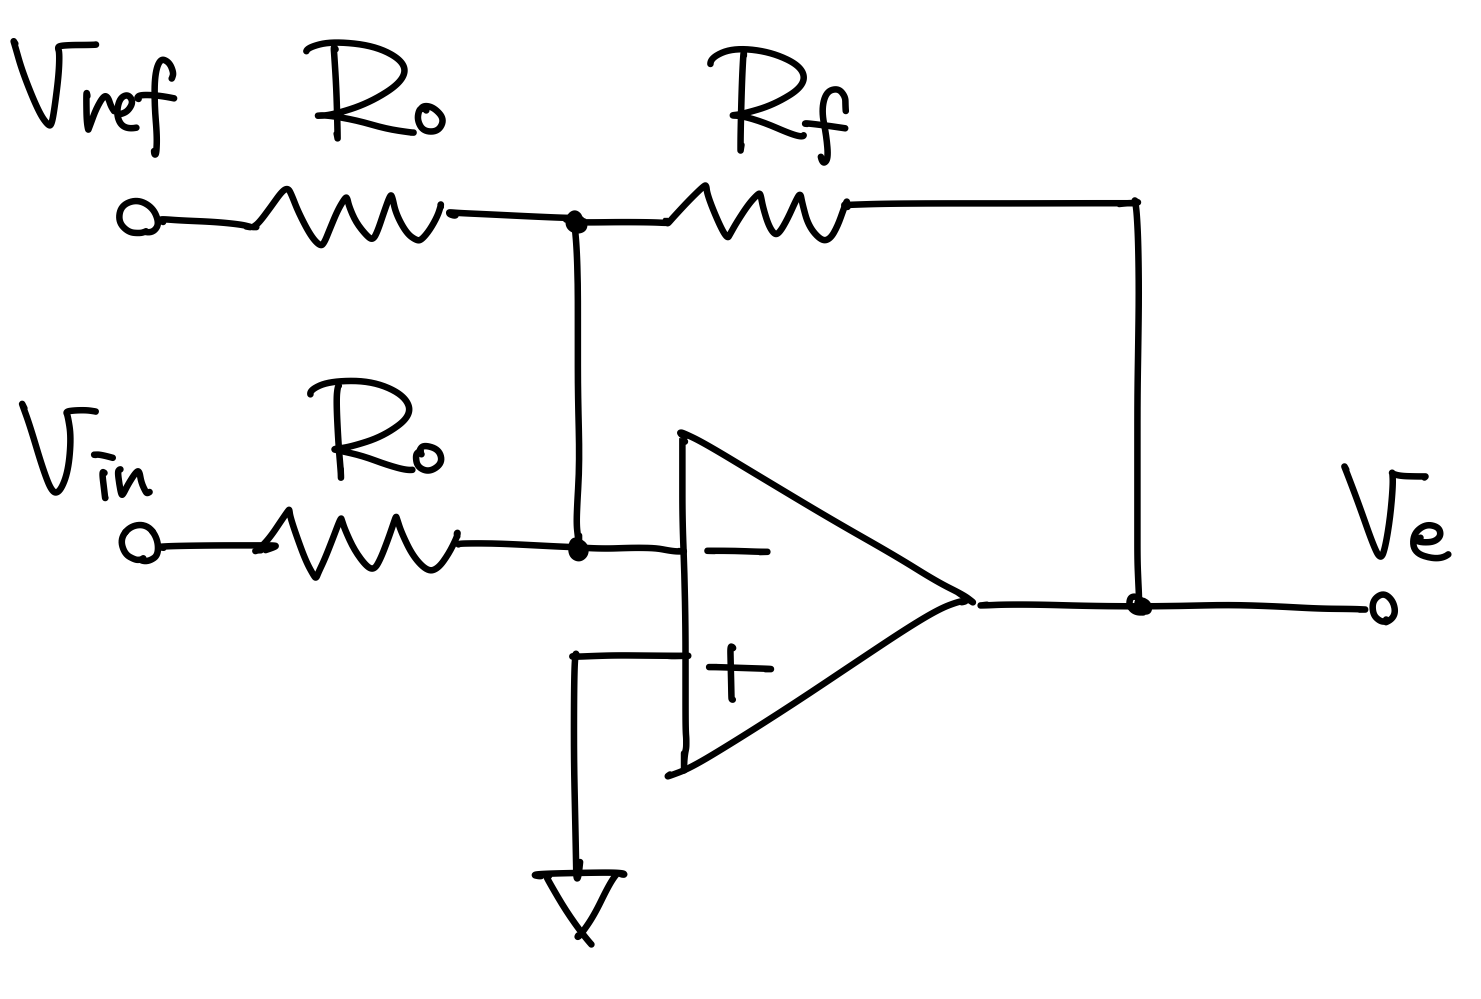
\includegraphics[width=0.8\columnwidth]{3_add.png}
          \caption{加算回路の概略図}\label{fig:3_add}
        \end{minipage}
        \begin{minipage}{0.45\columnwidth}
          \centering
          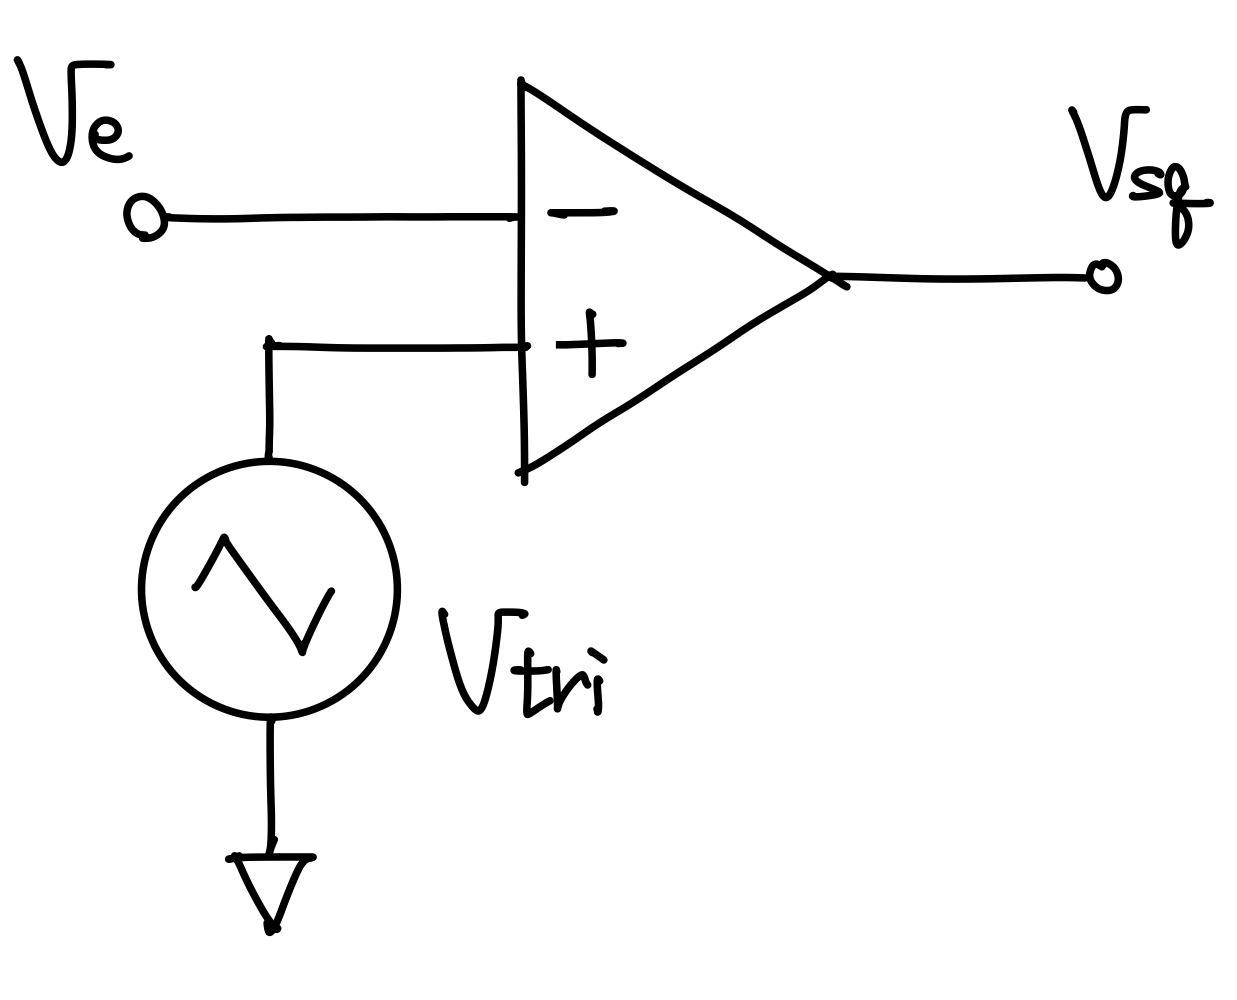
\includegraphics[width=0.8\columnwidth]{3_comp.png}
          \caption{比較回路の概略図}\label{fig:3_comp}
        \end{minipage}
      \end{figure}

    \subsubsection{フィードバック付きDCDCコンバータ}

      フィードバック付きDCDCコンバータの回路図を図\ref{fig:3_DCDC_add_comp}に示す.ここでは$V_\mathrm{in}$が表す電圧がこれまでと異なり,DCDCコンバータの入力電圧になることに注意されたい.図中のGは,DCDCコンバータ回路内のトランジスタのゲート端子を表す.


      \begin{figure}[htbp]
        \begin{center}
          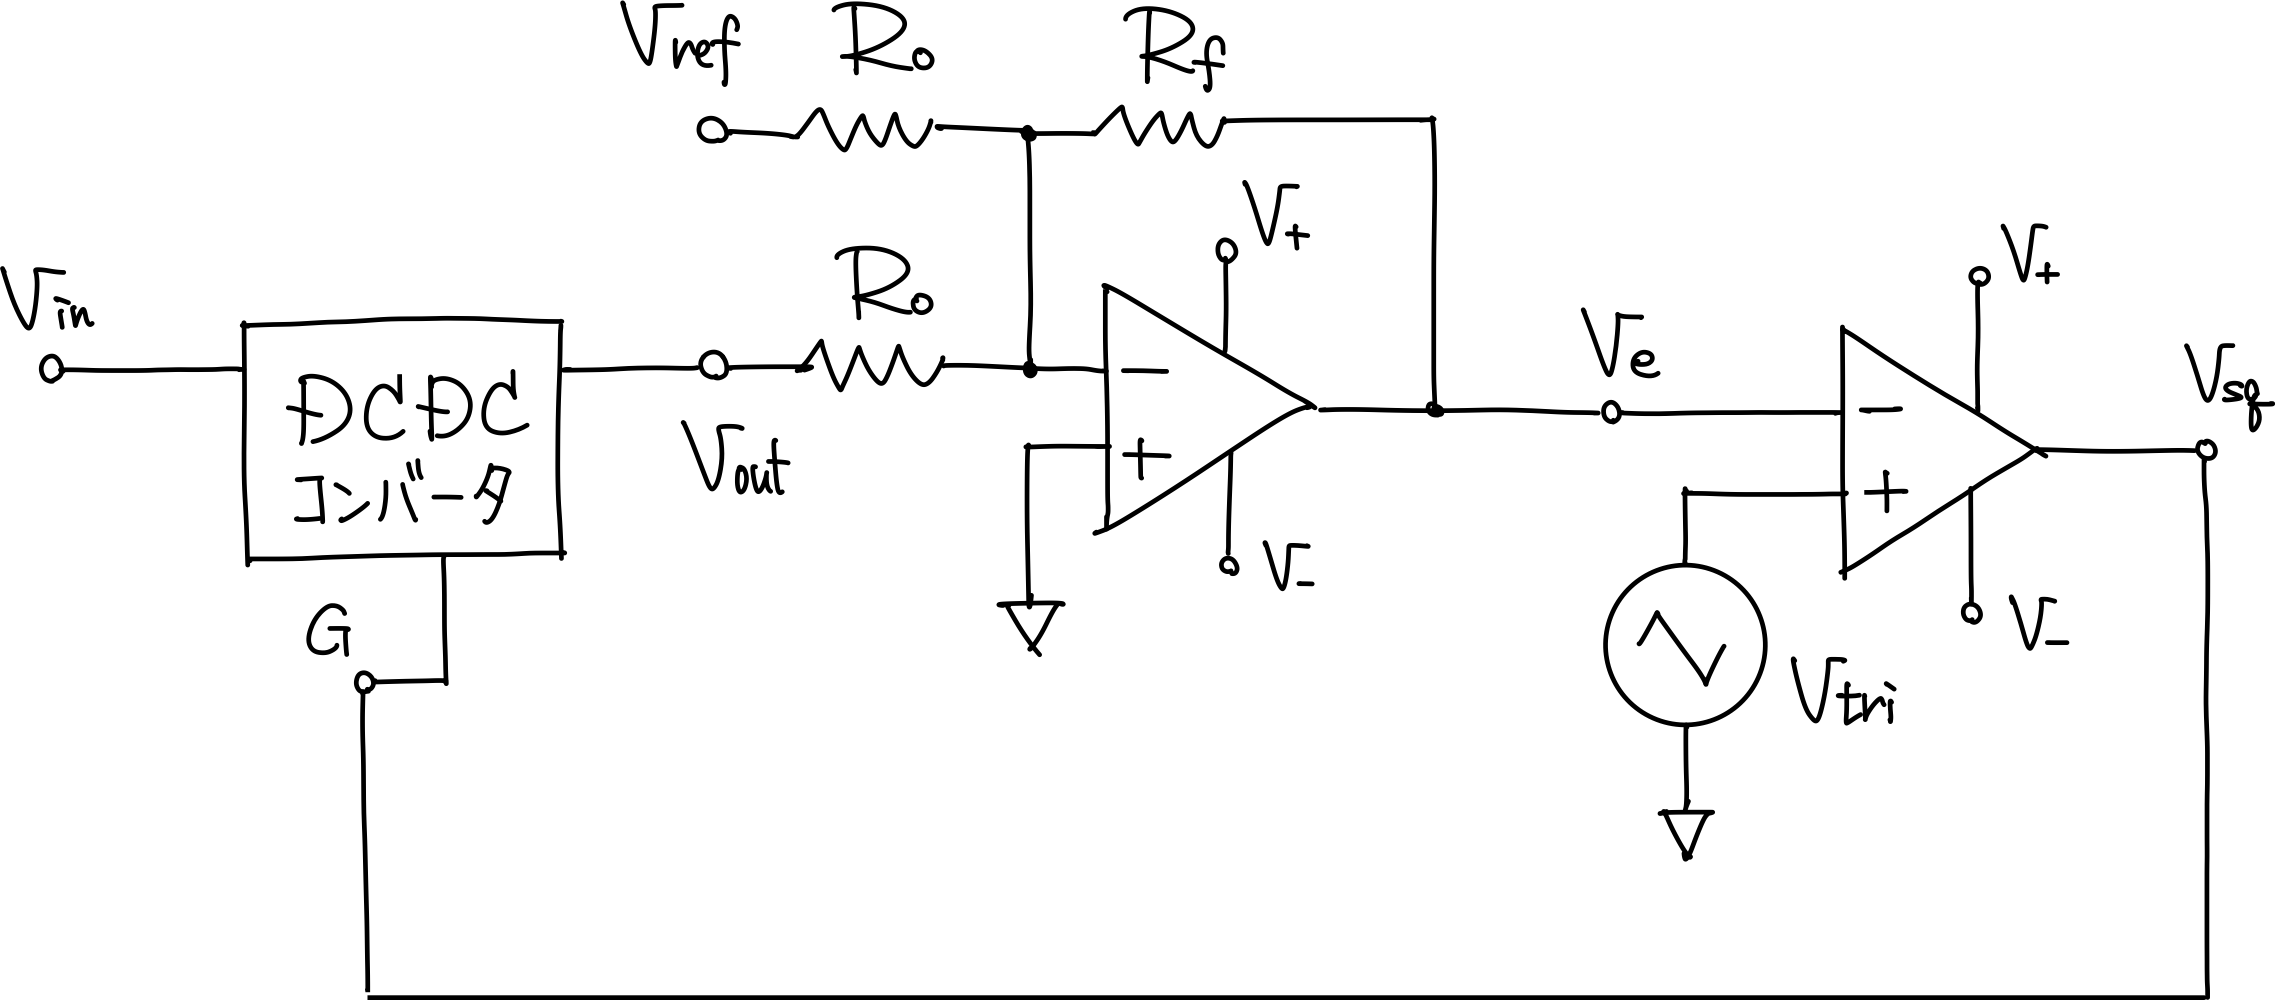
\includegraphics[width=0.8\columnwidth]{3_DCDC_add_comp.png}
          \caption{フィードバック付きDCDCコンバータ}\label{fig:3_DCDC_add_comp}
        \end{center}
      \end{figure}

      DCDCコンバータの入出力特性は

      \begin{equation}
        V_\mathrm{out} = -\frac{D}{1-D}V_\mathrm{in}
      \end{equation}
      であり,ここに式(\ref{eq:D})を代入して整理すると,

      \begin{equation}
        V_\mathrm{in} = - V_\mathrm{out} \cdot\frac{V_\mathrm{tri}-2K_\mathrm{fb}(V_\mathrm{ref}+V_\mathrm{out})}{V_\mathrm{tri}+2K_\mathrm{fb}(V_\mathrm{ref}+V_\mathrm{out})} \label{eq:3_DCDC_add_comp}
      \end{equation}
      という関係が成り立つ.これで,回路全体のパラメータを使って入出力特性を求めることができた.

  \subsection{方法}

    \subsubsection{実験1}

      図\ref{fig:3_add_comp_circ}に示す加算器と比較機を組み合わせた回路で,
      \begin{itemize}
        \item $R_0 = \SIs{10}{\kilo\ohm}$
        \item $V_\mathrm{ref} = \SIs{8.03}{\volt}$
        \item $V_\mathrm{tri} = \SIs{13}{\volt}$(peak-to-peak)
        \item (三角波の周波数) = $\SIs{50}{\kilo\hertz}$
        \item $V_+ = \SIs{15}{\volt}$
        \item $V_- = \SIs{-15}{\volt}$
      \end{itemize}
      とし,$K_\mathrm{fb} = -0.2, -0.51, -0.71$と変化させ,それぞれについて入力電圧$V_\mathrm{in}$と,方形波$V_\mathrm{sq}$のデューティ比$D$との関係を測定する.


      \begin{figure}[htbp]
        \begin{center}
          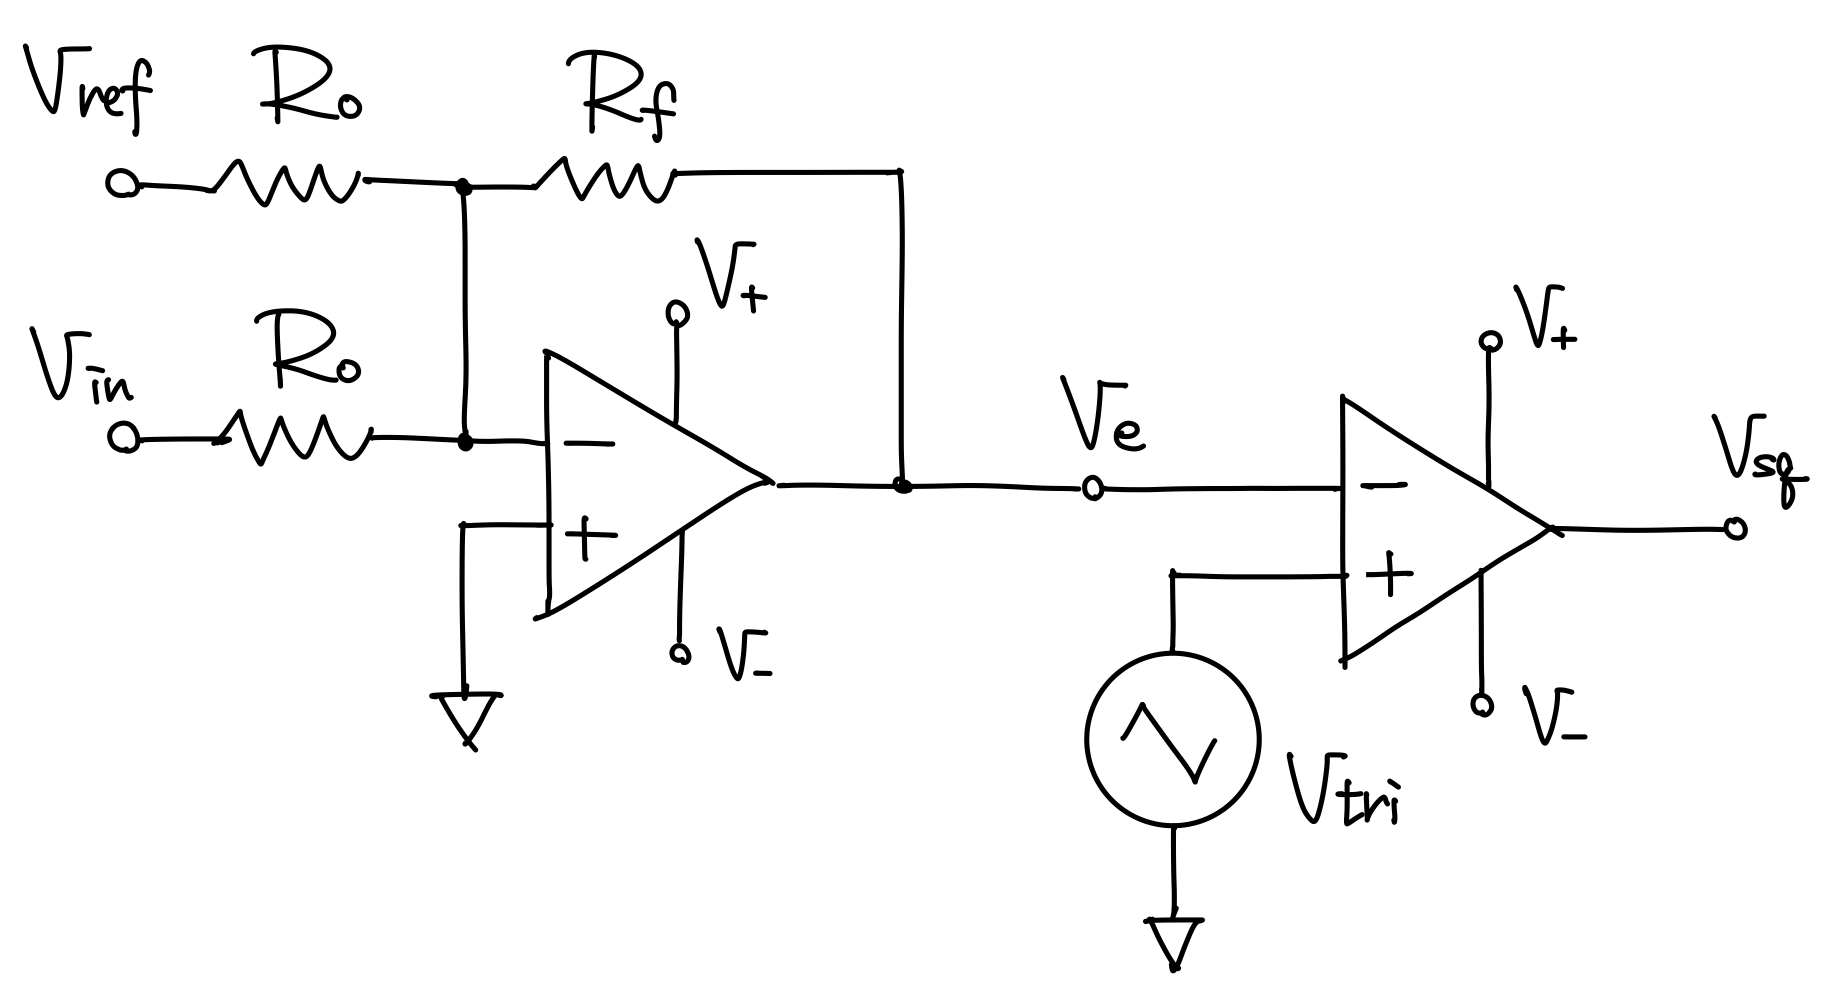
\includegraphics[width=0.8\columnwidth]{3_add_comp.png}
          \caption{実験1の回路図}\label{fig:3_add_comp_circ}
        \end{center}
      \end{figure}

    \subsubsection{実験2}

      測定対象の回路は図\ref{fig:3_DCDC_add_comp}で,実験1と同じパラメータで,$K_\mathrm{fb} = -0.2,-0.51$と変化させ,それぞれについて入力電圧と出力電圧とを測定する.

  \subsection{結果}

    \subsubsection{実験1}

      実験1の結果と,それぞれの理論線(式(\ref{eq:D}))を図\ref{fig:3_add_comp_result}に示す.

      \ref{fig:3_add_comp_result}からは,電圧が大きくなるにつれてデューティ比が直線的に大きくなることと,$K_\mathrm{fb}$が小さくなる(絶対値が大きくなる)につれてその直線の傾きが大きくなることが分かった.


      \begin{figure}[htbp]
        \begin{minipage}{0.45\columnwidth}
          \centering
          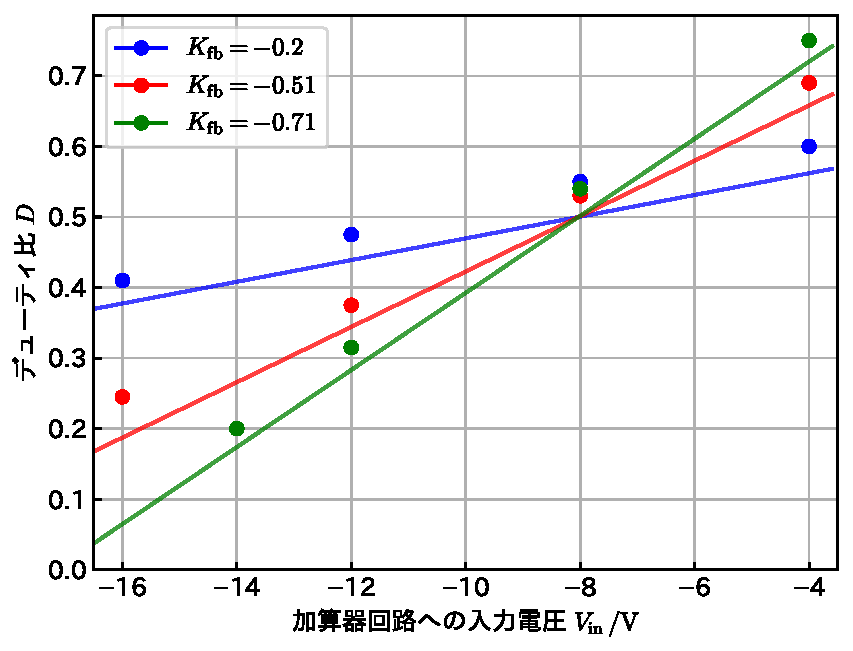
\includegraphics[width=0.8\columnwidth]{3_add_comp.pdf}
          \caption{実験1の結果}\label{fig:3_add_comp_result}
        \end{minipage}
        \begin{minipage}{0.45\columnwidth}
          \centering
          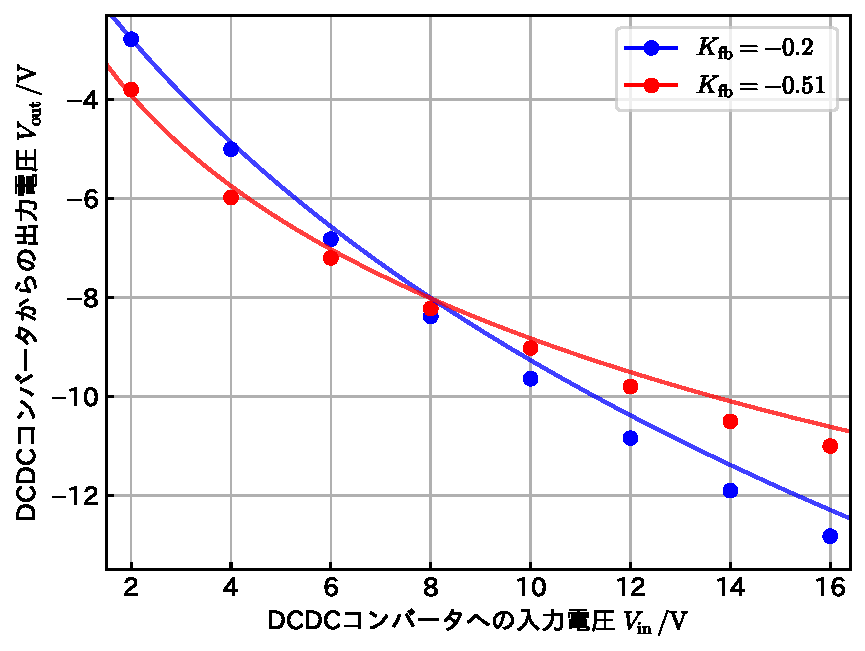
\includegraphics[width=0.8\columnwidth]{3_DCDC_add_comp.pdf}
          \caption{実験2の結果}\label{fig:3_DCDC_add_comp_result}
        \end{minipage}
      \end{figure}

    \subsubsection{実験2}

      実験2の結果とそれぞれの理論線(式\ref{eq:3_DCDC_add_comp})を図\ref{fig:3_DCDC_add_comp_result}に示す.

      $V_\mathrm{out}=\SIs{-8}{\volt}$付近を通る曲線の特性が見られ,また,$K_\mathrm{fb}$の絶対値が大きくなるほど曲線の傾きが小さくなることが観察できた.

  \subsection{考察}

    \subsubsection{実験1}

      図\ref{fig:3_add_comp_result}の測定点は理論線に沿って入るが,全体として理論値よりも大きい値であった.方形波を観察してみると図\ref{fig:oscillo}の紫色の線のような台形の波形が見られた.この波形の立ち上がり時間は$\SIs{10}{\text{\textmu}\second}$であり,これはオペアンプのスルーレートと一致していた.以上から,オペアンプのスルーレートによって方形波が\ruby{歪}{ひず}み,オン時間が長くなったことでデューティ比が大きくなったと考えられる.


      \begin{figure}[htbp]
        \begin{center}
          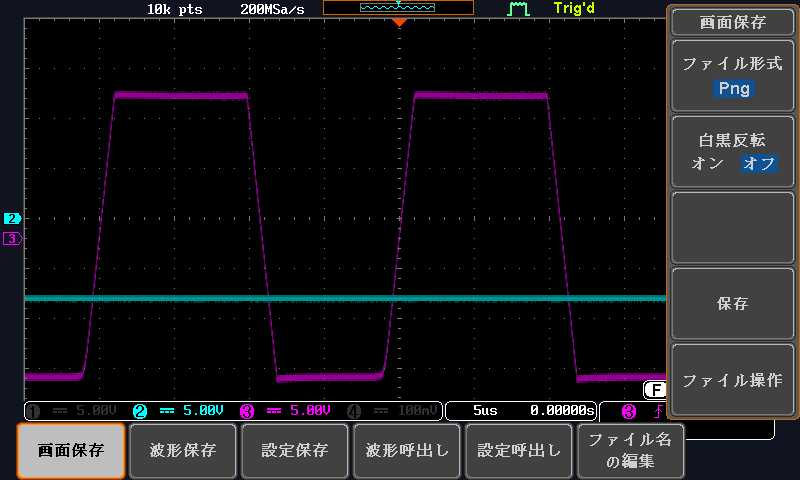
\includegraphics[width=0.5\columnwidth]{oscillo.jpg}
          \caption{$V_\mathrm{sq}$の波形}\label{fig:oscillo}
        \end{center}
      \end{figure}

    \subsubsection{実験2}
      実験1で述べたデューティ比の影響で,入力電圧が大きいところで出力電圧が理論値よりも大きくなっている.これを理論値に近づけるには,
      \begin{itemize}
        \item 周期に対してスルーレートが十分小さいような周波数域の三角波を利用する
        \item 加算器のフィードバック定数$K_\mathrm{fb}$の絶対値を大きくする
      \end{itemize}
      等が挙げられる.

\end{document}
